\documentclass[aps, prc, reprint, amsmath, groupedaddress, nofootinbib]{revtex4-1}
%\usepackage[compat=1.1.0]{tikz-feynman}
\usepackage[utf8]{inputenc}
\usepackage{hyperref}
\usepackage{amsmath}
\usepackage{amssymb}
\usepackage{amsfonts}
\usepackage{tabularx}
\usepackage{booktabs}
\usepackage{graphicx}
\usepackage{color}
\usepackage{multirow}
\usepackage{verbatim}
\usepackage[inline]{enumitem}
\graphicspath{{fig/}}
\definecolor{theblue}{RGB}{0,50,230}
\usepackage{appendix}
\hypersetup{
  colorlinks=true,
  linkcolor=theblue,
  citecolor=theblue,
  urlcolor=theblue
} 


\begin{abstract}
A Monte-Carlo simulation is a useful tool in the phenomenological study of the jets and heavy quarks in the heavy-ion collisions.
However the multiple-scattering induced gluon radiation--important at high energy--cannot be factorized into independent processes due to the coherence effect and it is hard to be implemented in a Monte-Carlo way.
Many existing implementations capture qualitatively behaviors or focus on certain limits, but it is important to study if an approach quantitatively agree with the current knowledge from theory.
In this work, we compared three specific implementations to the perturbative calculation.
In a static medium, we found that a particular implementation well reproduce the semi-analytic calculations of the parton radiative energy loss.
The impacts of an expanding medium, running coupling and mass effect are also discussed.
This implementation is not only a good surrogate model of the theory, but also a tunable one that can calibrated to experimental data. 
By controlling the modeling uncertainty between the Monte Carlo implementations and the theory, a more meaningful extraction of the transport properties of energetic partons inside a quark-gluon plasma can be performed in the future.
\end{abstract}

\begin{document}
\title{Calibrating Monte-Carlo implementations of parton radiative energy loss to theoretical limits.}
\author{Weiyao Ke}
\author{Steffen A.\ Bass}
\affiliation{Department of Physics, Duke University, Durham, NC 27708-0305}
\date{\today}
\maketitle 

\section{Introduction}
The study of hard probes in relativistic heavy-ion collisions is moving towards the precision era thanks to the future experimental upgrades \cite{ATLAS-Collaboration:2012iwa,Abelevetal:2014dna,STAR:upgrade-hf,Adare:2015kwa,CMS:2017dec}.
On the phenomenology side, it is imperative to revisit our assumptions and approximations to do a more meaningful model-to-data comparison to extract interested properties of the quark-gluon plasma (QGP) via hard probes.
Systematic calibration of medium evolution models on soft-observables have shown success in extracting the temperature dependent shear and bulk viscosity, benefiting from both high accuracy data and models with well controlled uncertainties that allow parameter fine-tuning \cite{Bernhard:2016tnd, Bernhard:2018hnz}.
Applying this model calibration to the extraction of jets and heavy quark transport parameters, we encountered new difficulties. 
First, the transport coefficients have both temperature and momentum dependences, increasing the complexity of uncertainty parametrization \cite{Xu:2017obm}.
Second, the model (theory) uncertainties are large. 
Model uncertainties not only originate from different assumptions that define different theories \cite{CaronHuot:2010bp, Rapp:2018qla}, but also hide in the numerical approximations of the theory.
Because theory uncertainty can obscure the physical statement of the extracted parameters, we need to put it under control or at least estimate its impact before future model-to-data comparisons.
For studying the impacts of using different theory assumptions, such as whether the nature of the interaction is perturbative or non-perturbative or even both, there are on-going efforts from the JETSCAPE collaboration to interface different theories in a unified way \cite{Cao:2017zih, Kauder:2018cdt}.
In this work, we aim to reduce and control the uncertainty that comes from the numerical implementation of a specific type of theory, which is the transport theory based on perturbative QCD.

The application of perturbative QCD to partonic transport in heavy-ion collisions has been developed over the years \cite{Arnold:2002zm}.
In a near equilibrium medium, energetic partons interact with medium through both elastic (collisional) and inelastic (medium induced gluon radiation) processes at leading order \cite{Ghiglieri:2015ala}.
Because of the complexity of the medium dynamics in realistic collisions, Monte Carlo implementations of the pertubative physics are developed for phenomenology.
At high energy, the largest uncertainty that is introduced in these Monte Carlo generators comes from different treatments of the gluon radiation since it is the dominant source of energy loss at high energy.
For such radiation in a dense medium, the QCD Landau-Pomeranchuk-Migdal (LPM) effect is important, where multiple scatterings during the radiating gluon formation time act coherently to suppress the radiation spectrum \cite{PhysRev.103.1811,Wang:1994fx,Zakharov:1996fv,Baier:1996kr}.
Therefore, a medium induced radiation becomes an effectively $n$-body to $(n+1)$-body process that extends in space-time.
This feature is particularly difficult to be accurately implemented in a Monte-Carlo way, where interactions are usually treated as local.
To simplify the problem while still keep the essential qualitative natures such as path-length dependence and spectrum shape, different methods are used in numerical studies \cite{Djordjevic:2008iz,Cao:2013ita,ColemanSmith:2012vr,Xu:2004mz, Zapp:2011ya, Gossiaux:2012cv,Park:thesis}.
In this work we compare quantitatively three implementations with different physical motivations to the knowledge from the perturbative calculations in idealized limits \cite{Arnold:2008zu,Arnold:2009mr}.
Among them, a slightly modified approach based the method that takes into account gluon multiple scatterings works remarkably well \cite{Zapp:2011ya}.
This method, referred to as the ``Modified Rescattering" approach, well reproduces the analytic calculations of energy loss as function of coupling constants, temperatures, parton energies and path lengths.
We also introduce parameters to control its finite- and infinite-size behaviors separately.
This way the parameters can be fine-tuned to match the theory on the one hand; on the other hand, they can also be calibrated to experimental data.
The performance of the theory can therefore be measured quantitatively on the landscape of this parameter space in future statistical analysis.

This paper is organized as follows. Section \ref{section:qual} reviews the qualitative spectrum of the medium induced radiation.
In Section \ref{section:MC}, three Monte Carlo implementations of the radiative processes are discussed. 
Semi-analytic results to which the Monte Carlo simulations are compared are briefly summarized in Section \ref{section:Theo}.
The major results are discussed in Section \ref{section:results}.
Finally, we discuss in Section \ref{section:disscuss} the running coupling effect, expanding medium effect and the mass (dead-cone) effect in the ``Modified Rescattering" implementation. Section \ref{section:summary} is a brief summary.



\section{Qualitative features of the suppression}\label{section:qual}
In this section, we introduce the qualitative features of the medium induced radiation following the discussion in \cite{Baier:1996kr}.
A radiated gluon stays in coherence with the mother partons for a finite amount of time determined by the uncertainty principle $\Delta t \sim 1/\Delta E$. 
$\Delta E$ is the different between the initial mother patron energy $E$ and the energies of the final state daughter partons.
The formation time is then,
\begin{eqnarray}\label{eq:tau_1}
\tau_f = \frac{2(1-x)\omega}{k_\perp^2+(1-x)m_g^2},
\end{eqnarray}
where $x = \omega/E$, $m_g^2=m_D^2/2 \sim \alpha_s T$ is the gluon thermal mass squared.
The formation time looks like $\omega/(\alpha_s T^2)$ for a collinear splitting.
Meanwhile, the gluon can keep interacting with the dense medium via elastic collisions with a rate $R_{g} = 1/\lambda_g$ that scales like $\alpha_s T$. 
Therefore, the number of rescatterings within the formation time $N \sim \tau_f R_g \sim \omega/T$ may not be a small number for gluon with energy comparable or larger than the medium temperature.
Since rescatterings also change the transverse momentum $k_\perp$ of the gluon relative to the mother parton, a self-consistent formation time estimation is required.
Given that elastic scattering increases the average $k_\perp^2$ by an amount $\hat{q}_g\tau_f$ where $\hat{q}_g = d\langle k_\perp^2\rangle/dt$ is the gluon transport coefficient, the self-consistent condition is
\begin{eqnarray}\label{eq:tau_n}
\tau_f \sim \frac{2(1-x)\omega}{\hat{q}_g\tau_f} \longrightarrow \tau_f \sim \sqrt{\frac{2(1-x)\omega}{\hat{q}_g}}
\end{eqnarray}
The inverse of the formation time measures the rate of a gluon being separated from the mother parton.

The medium induced gluon radiation is understand as follows. 
A virtual gluon with energy $\omega$ and transverse momentum $k_\perp$ splits from the mother parton with the probability given by the vacuum splitting function ($P(x) \sim \alpha_s/x$).
If its formation time is smaller than the mean-free-path of elastic scattering (the Bethe-Heitler region), it is put on shell with the rate $1/\lambda_g$; otherwise multiple rescatterings put it on-shell with a rate $1/\tau_f$ (the LPM region).
As a result, the differential radiation rate is,
\begin{eqnarray}\label{eq:LPM}
\frac{dP}{dt d\omega} \sim \begin{cases}
 \frac{\alpha_s}{\omega} \frac{1}{\lambda_g} \sim \alpha_s^2  \frac{T}{\omega}, \hfill \tau_f \lesssim \lambda_g\\
 \frac{\alpha_s}{\omega} \frac{1}{\tau_f}\sim \alpha_s \sqrt{\frac{\hat{q}_g}{T^3}} \left(\frac{T}{\omega}\right)^{3/2}, \hfill \lambda_g \lesssim \tau_f
\end{cases}
\end{eqnarray}
We note first that in the leading order picture, the LPM effect modifies the single gluon emission rate. 
It does not introduce correlations between subsequent emissions which are higher order effects \cite{Arnold:2016jnq}.
Second, the emission rate at a certain time receives coherent contributions from the collision centers whose locations extend about $\tau_f$ along the path of the mother parton.
Therefore in a thin medium of size $\lambda_g < L< \tau_{f,\textrm{max}} \sim \sqrt{E/\hat{q}_g}$ with limited number of scattering centers, the second line of Equation \ref{eq:LPM} is replaced by,
\begin{eqnarray}
\frac{dP}{dt d\omega} \sim 
 \frac{\alpha_s C_R}{\omega} \frac{1}{\min\{\tau_f,L\}}, \hfill \lambda_g < \tau_f
\end{eqnarray}
The radiative energy loss is obtained by integrating over the differential rate times the gluon energy. 
For the case of an infinite medium, this is
\begin{eqnarray}\label{eq:dE-Linf}
\Delta E/\Delta L \sim \alpha_s^2 \sqrt{ET^3}
\end{eqnarray}
For a thin medium, the LPM effect leads to the non-linear path length $L$ dependence of the energy loss
\begin{eqnarray}\label{eq:dE-Lfinite}
\Delta E \sim \alpha_s \hat{q} L^2
\end{eqnarray}
When the path length exceed the $\tau_{f,\textrm{max}}$, $\Delta E$ should smoothly transit to the behavior given by Equation \ref{eq:dE-Linf}.

\section{Different Monte-Carlo implementations}\label{section:MC}
Despite there are many ideas of implementing LPM effects,
we compare only those approaches that treat this effect non-locally and result in a non-linear path length dependence.
The framework we worked in is the {\tt Lido} model \cite{Ke:2018tsh}. 
It is originally designed for heavy quark transport inside a QGP. 
In this section, we turn off all quark mass effects (phase-space, matrix-elements) to study light quark first.
The {\tt Lido} model is based on elementary ($2\rightarrow2$) elastic and inelastic pQCD scatterings. 
The inelastic processes include both gluon radiation ($2\rightarrow 3$) and gluon absorption ($3\rightarrow 2$) processes using an improved Gunion-Bertsch approximated matrix-element \cite{Fochler:2013epa,Uphoff:2014hza}.
For the comparison to theory calculations, we only turn on the $2\rightarrow 3$ channel for the high energy quark and the $t$-channel in the elastic scatterings.
Next, we introduce three different LPM effect implementations in detail.

\paragraph*{``Coherence factor" approach} This first approach is the old one used in the {\tt Lido} model. 
It inherits from early works using a radiation improved Langevin equation \cite{Cao:2013ita} and is also implemented in the Linearized-Boltzmann-Transport-Model \cite{Cao:2016gvr,Cao:2017hhk}. 
One can refer to Appendix \ref{app:consistency} that the formula used in {\tt Lido} reduces to the one used in \cite{Cao:2013ita} when the momentum transfer from the medium is much smaller than the transverse momentum of the radiated gluon.
The incoherent limit of the rate is calculated using $2\rightarrow 3$ Gunion-Bertsch cross-section $\sigma_\textrm{GB}$,
\begin{eqnarray}\label{eq:GB-rate}
\Gamma = \frac{1}{2E_1}\int\frac{f_i(p_2)d\vec{p_2}^3}{(2\pi)^3 2p_2}2\hat{s}\int d\hat{t}\frac{d\vec{k}^3}{(2\pi)^3 2k}\frac{d\sigma_{\textrm{GB}}}{d\hat{t}d\vec{k}^3}
\end{eqnarray}
The ``Coherence factor" appraoch implements LPM suppression by multiplying a time-dependent coherence factor to the final state gluon phase space integration in Equation \ref{eq:GB-rate},
\begin{eqnarray}
\frac{d\vec{k}^3}{(2\pi)^3 2k} \rightarrow \frac{d\vec{k}^3}{(2\pi)^3 2k} 2\left[1-\cos\left(\frac{t-t_0}{\tau_f}\right)\right]
\end{eqnarray}
The modified rate dependents on the time separation $\Delta t = t-t_0$ which is the time elapse from the last gluon emission.
The value of $\Delta t$ is only determined at run-time,
but we can still estimate its order-of-magnitude from the following condition:
\begin{eqnarray}
1 \sim \int_0^{\Delta t}\Gamma(t) dt,
\end{eqnarray}
which means that the probability to have one radiation within $\Delta t$ should be of order $1$, as required by the definition of $\Delta t$.
By dimensional analysis, this gives $\Delta t \sim 1/\alpha_s T$.
We see that this prescription indeed suppresses the spectrum when the formation time is much greater than the mean-free-path. 
However, multiple scatterings are not included since gluons are always produced in $2\rightarrow3$ processes.
Moreover, it introduces correlation between the locations of vertices of subsequent emissions;
especially, no matter how soft the previous radiation is, it affects the next radiation in the same way through $\Delta t$.

The next two approaches both taken into account the gluon multiple scattering effect motivated by the implementation \cite{Zapp:2011ya}.
A gluon is first sampled from an $2\rightarrow3$ inelastic scattering at time $t=t_0$, but it is not regarded as ``formed" immediately. 
This gluon keeps interacting with the medium via elastic processes that change the gluon transverse momentum $k_{\perp,n}$ and formation time $\tau_{f,n}$ via Equation \ref{eq:tau_1}.
Here, the subscripts $n$ denote the quantities calculated after the $n$-th rescattering.
This continues until the time elapse since $t_0$ just exceeds the gluon formation time,
\begin{eqnarray}\label{eq:self-consisten-condition}
\tau_{f, n} < t-t_0 < \tau_{f, n-1}.
\end{eqnarray}
After this amount of time, the gluon is considered to have lost coherence with the mother parton.
The formation time determined in this way reproduces the self-consistent condition of Equation \ref{eq:tau_n}.
Even with this self-consistent formation time, it is still tricky to introduce the correct suppression, so we discussed and compared the following two approaches. 

\paragraph*{``Blocking radiation" approach}
An attempt to introduce suppression is by requiring that no other radiation is allowed within $t-t_0$ showed in Equation \ref{eq:self-consisten-condition}, referred to as the ``blocking radiation" approach in this paper.
It certainly suppresses the radiation rate and also results in a non-linear path length dependence of the energy loss; however, a closer examination reveals its problems.
First of all, it again introduces correlations between subsequent emission vertices.
But the biggest problem is that it does not alter the spectrum shape, because though each suppression is delayed by $\tau_f$, it is generated according to the incoherent rate. 
It only suppresses the $2\rightarrow 3$ spectrum by an overall factor $1/N$ that reduces $N$ possible inelastic collisions to a single one,
\begin{eqnarray}
N \sim \frac{\left\langle\tau_{f,N}\right\rangle}{ \lambda_{\textrm{inel}}}.
\end{eqnarray}
This approach is certainly not so ideal, but we still keep it as an example for comparison.

\paragraph*{``Modified rescattering" approach} Finally, we implement another approach modified from the one studied in \cite{Zapp:2011ya,Park:thesis,Park:2016jap}.
It is designed to reproduce the qualitative spectrum of Equation \ref{eq:LPM} and does not introduce extra correlations between different emission vertices. 
Comparing to \cite{Zapp:2011ya}, we avoid the use of quantities such as the mean-free-path $\lambda$ or the number of scattering centers, since these quantities are sensitive to the regularization of the matrix-elements. 
The substitute for $\lambda$ is an ``effective" mean-free-path $\tilde{\lambda}$ defined by,
\begin{eqnarray}\label{eq:effmpf}
\tilde{\lambda} = \frac{m_D^2}{\hat{q}_g(\omega, T)}
\end{eqnarray}
The advantages are not only that $\tilde{\lambda}$ is less sensitive to regularization, but also that it can be applied to other models that do not rely on individual scatterings, such as the radiation-imporved Langevion equation.
This is particular useful if one would like to absorb small angle scatterings into a diffusion equation \cite{Ghiglieri:2015ala}, then $\hat{q}$ will be the sum of a large-angle scattering contribution and a diffusion contribution.

Here are the detailed steps of the implementation,
\begin{itemize}
\item[1.] In a time step $\Delta t$, the mother parton undergoes inelastic scatterings with probability $\Gamma\Delta t$. $\Gamma$ is the incoherent rate from Equation \ref{eq:GB-rate}.
\item[2.] If a gluon $i$ is sampled at $t_{i,0}$, it is appended to a ``pre-gluons" list associated to the mother parton. But its energy is not carried away from the mother.
\item[3.] Loop over the ``pre-gluons" list. 
\begin{itemize}
\item[3.1] If $\tau_f > t-t_{i,0}$, evolve this gluon (elastic scatterings, diffusion, or both). Recalculate its formation time.
\item[3.2] If $\tau_f < t-t_{i,0}$, accept it with probability $p = \min\{1, a\}$. Accepted gluons are formed and its energy is subtracted from the mother. Otherwise, they are removed from the list without causing energy loss.
\end{itemize} 
\item[4.] Repeat for the next time step.
\end{itemize}
Here, we use the term ``pre-gluons" to denote those gluons that are not fully formed.
One mother parton can carry an arbitrary number of ``pre-gluons" and there are no correlations among them.
The formation time is determined as Equation \ref{eq:self-consisten-condition}, so on average $\tau \sim \sqrt{\omega/\hat{q}}$.
The acceptance parameter $a$ is,
\begin{eqnarray}
a = \frac{\tilde{\lambda}}{\tau_f} \sqrt{1-x+\frac{C_A}{C_F}x^2}
\end{eqnarray}  
The factor $\tilde{\lambda}/\tau_f$ guarantees that the radiation spectra in the LPM region scales like the one given in Equation \ref{eq:LPM}; the square root term is motivated by the form leading-log results in \cite{Arnold:2008zu}.

It worth mention that the formation time in Equation \ref{eq:tau_1} and the effective mean-free-path Equation \ref{eq:effmpf} is only an order of magnitude measure of the coherence effect. 
These relations can be fine tuned to best reproduce the quantitative theory calculations to be discussed in the next section.
For this purpose, we introduces the following tunable relations,
\begin{eqnarray}\label{eq:tune}
\nonumber
\tau_f' &=& C_1 \frac{2(1-x)\omega}{k_\perp^2+(1-x)m_g^2} \\
p &=& \min\left\{1, \frac{C_2}{\sqrt{C_1}} a\right\}
\end{eqnarray}
The parameters $C_1$ and $C_2$ are unities by default and are designed such that $C_1$ and $C_2$ controls the finite- and infinite-size behaviors separately. 
This is possible by realizing that the comparison between medium length and the formation time solely determines the finite size effect; while the acceptance condition alone controls the strength of the suppression in an infinite medium.
Though it is possible to fine tuning these parameters to increase the similarity between the Monte Carlo simulation and the theory, we are going to show in Section \ref{section:results} that the default setting $C_1 = C_2 = 1$ already closely mimics the theory.
These parameters are also handles to deform the behavior of the Monte-Carlo away from the underlying theory in a controllable way.
Their values fine tuned to experiments are not necessarily the same as those tuned to theory. 
The parameter space $(C_1, C_2)$ is the map showing the distance from the theory to the phenomenology model required by data.

\begin{figure*}
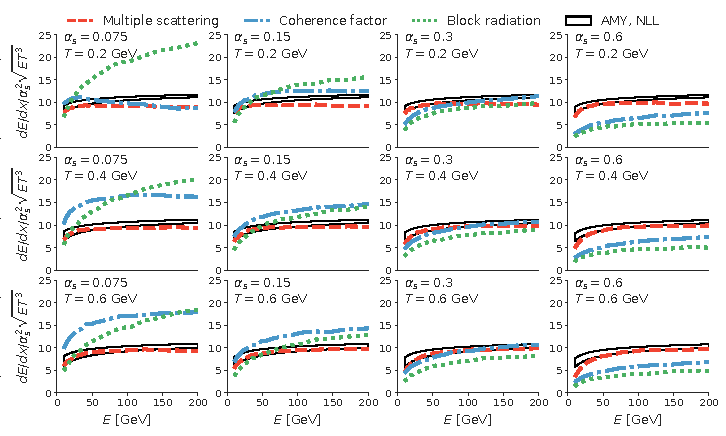
\includegraphics[width=\textwidth]{Eloss_infinite.pdf}
\caption{Energy loss per unit path lengh $dE/dx$ as a function of energy $E$, temperature $T$ and coupling constant $\alpha_s$. Each column corresponds to $\alpha_s = 0.075, 0.15, 0.3$, and $0.6$ (from left to right). Each column corresponds to $T = 0.2, 0.4$, and $0.6$ GeV (from top to bottom). $dE/dx$ is divided by the expected scaling $\alpha_s^2 \sqrt{ET^3}$. The calculations from ``Modified rescattering", ``Coherence factor", and ``Block radiation" approaches are the red-dashed lines, blue-dash-dotted lines, and green-dotted lines respectively. The AMY NLL results are denoted as black boxes.}
\label{fig:eloss-inf}
\end{figure*}

\begin{figure*}
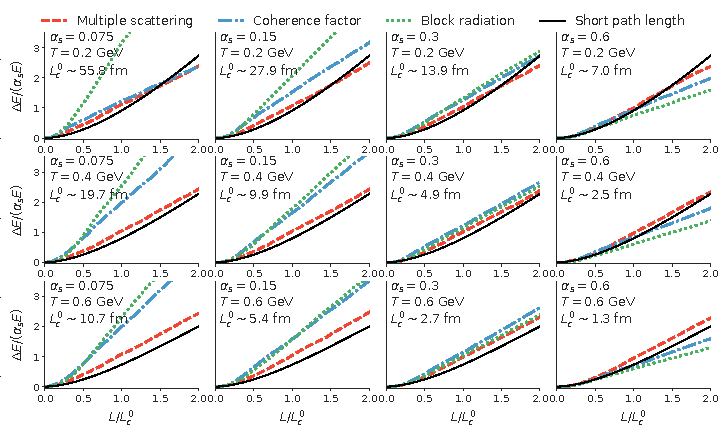
\includegraphics[width=\textwidth]{Eloss_Ldep.pdf}
\caption{Energy loss $\Delta E$ as a function of path length $L$, temperature $T$ and coupling constant $\alpha_s$. Each column corresponds to $\alpha_s = 0.075, 0.15, 0.3$, and $0.6$ (from left to right). Each column corresponds to $T = 0.2, 0.4$, and $0.6$ GeV (from top to bottom). $\Delta E$ is scaled by $\alpha_s E$ and $L$ is scaled by an estimated critical path length $L_c^0 = \sqrt{E/\hat{q}_0}$, $\hat{q}_0\sim 4\pi C_A\alpha_s^2 \times 1.28 T^3$. The calculations from ``Modified rescattering", ``Coherence factor", and ``Block radiation" approaches are the red-dashed lines, blue-dash-dotted lines, and green-dotted lines respectively. The analytic results for thin medium are denoted as black solid lines.}
\label{fig:eloss-ldep}
\end{figure*}

\begin{figure}
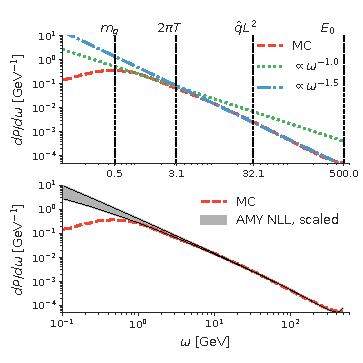
\includegraphics[width=\columnwidth]{spectrum.pdf}
\caption{Radiated gluon spectrum in an infinite medium from a quark $E=500$ GeV, $\alpha_s = 0.1$. The top plot shows the spectrum (red-dashed line) and power law fit (green-dotted and blue-dash-dotted lines) in different gluon energy ($0<\omega < E$) regions, separated by energy scale $m_g$, $\hat{q}_0\lambda_g^2 \sim 2\pi T$. The middle plot is the same simulation compared to the incoherent spectrum and the AMY semi-analytic result. The bottom plot is the ratio between the Monte-Carlo simulation and the semi-analytic calculation.}
\label{fig:spectrum}
\end{figure}
\section{Semi-analytic formula for radiative energy loss}\label{section:Theo}
The main purpose of this study is to gauge Monte Carlo implementations using theories.
Here we use the (semi-)analytic results from two theoretical works where medium induced gluon radiation is solved in an infinitely large medium (to next-to-leading-log accuracy) and in a thin medium (to leading-log accuracy).
For readers convenience, we briefly summarize their results in this section.

In an infinite static medium, the formula for gluon radiation spectrum (we only use the one for gluon splitting from a quark) is derived in \cite{Arnold:2002zm,Arnold:2003zc},
\begin{eqnarray}\label{eq:AMY-1}
\nonumber
\frac{dP_{q\rightarrow qg}}{dt dx} &=& \frac{1}{2E\nu_q} \frac{\alpha_s d_F P_{q\rightarrow qg}(x)}{2x^2(1-x)^2}\int\frac{d^2\vec{h}}{(2\pi)^2}2\vec{h}\cdot \mathfrak{Re} \vec{F} \\
&\times& [1+f_g(xp)][1-f_q((1-x)p)],
\end{eqnarray}
where $\vec{F}(\vec{h}; p, x)$ satisfies the following equation,
\begin{eqnarray}\label{eq:AMY-2}
\nonumber
2\vec{h} &=& i\frac{h^2 \vec{F}(\vec{h})}{p^3 2x(1-x)} \\
\nonumber
&+& g^2\int \frac{dq_\perp^2 \mathcal{A}(q_\perp^2)}{(2\pi)^2}\left\{\frac{C_A}{2}\left[\vec{F}(\vec{h}) - \vec{F}(\vec{h}+p\vec{q}_\perp)\right]\right. \\
\nonumber
&& \phantom{ssss} + \left(C_F - \frac{C_A}{2}\right)\left[\vec{F}(\vec{h}) - \vec{F}(\vec{h}-xp\vec{q}_\perp)\right] \\
&& \phantom{sssssss} + \left. \frac{C_A}{2}\left[\vec{F}(\vec{h}) - \vec{F}(\vec{h}-(1-x)p\vec{q}_\perp)\right] \right\}.
\end{eqnarray}
The collision kernel of a gluon in a thermalized QGP is,
\begin{eqnarray}
\mathcal{A}(q_\perp^2) = \frac{T m_D^2}{q_\perp^2(q_\perp^2+m_D^2)}.
\end{eqnarray}
The exact solution can be obtained numerically, but the author of \cite{Arnold:2008zu} obtained a semi-analytic solution to the next-to-leading-log ($[\ln(E/T)]^{-1}$) accuracy, which comes handy to calibrate the Monte Carlo generators,
\begin{eqnarray}\label{eq:AMY-NLL}
\frac{dP_{q\rightarrow qg}^{\textrm{NLL}}}{dt dx} &=& \frac{\alpha_s}{2\pi}\frac{ d_F P_{q\rightarrow qg}(x)}{\sqrt{2}\nu_q x(1-x)E} m_D^2 \hat{\mu}_\perp^2(x),
\end{eqnarray}
with $\hat{\mu}_\perp^2(x)$ determined by the self-consistent condition,
\begin{eqnarray}\label{eq:AMY-sf}
\nonumber
\hat{\mu}_\perp^2 && = \frac{gT}{m_D} \sqrt{\frac{2x(1-x)E}{\pi T}}\left\{
\frac{C_A}{2}(1-x)^2\ln\left[\frac{\xi\hat{\mu}_\perp^2}{(1-x)^2}\right] + \right. \\
&&\left.\left(C_F-\frac{C_A}{2}\right)x^2\ln\left(\frac{\xi\hat{\mu}_\perp^2}{x^2}\right) + \frac{C_A}{2}\ln(\xi\hat{\mu}_\perp^2)\right\}^{\frac{1}{2}}.
\end{eqnarray}
And $\xi\approx9.09916$ is a constant. Since we do not use quantum statistics in the Monte Carlo generators, we have dropped the Bose enhancement and the Pauli blocking factors in Equation \ref{eq:AMY-NLL}.
The NLL result is a good approximation when $\ln(xE/T)$ is large. 
It shoots above the numerical solutions with some universal behaviors when $\ln(xE/T)$ is small.
We estimate this uncertainty by including an artificial multiplicative correction factor to Equation \ref{eq:AMY-NLL}, 
\begin{eqnarray}\label{eq:correction}
R_{\textrm{corr}} = \frac{1}{1+0.8\left(xE/T\right)^{-0.7}}.
\end{eqnarray}
It mimic the systematic deviation of Equation \ref{eq:AMY-NLL} from the numerical solution. 
Later we will see that for the relevant temperatures and parton energy larger than $10$ GeV, this is not a big effect for the energy loss.
To better see the physical interpretation of this formula, we also quote the lead-log result for $\hat{\mu}_\perp^2(x)$ from \cite{Arnold:2008zu},
\begin{eqnarray}\label{eq:AMY-LL}
\nonumber
\hat{\mu}_{\perp, \textrm{LL}}^2 = \frac{gT}{m_D} \sqrt{\frac{2x(1-x)E}{\pi T}}\left\{
\frac{C_A}{2}(1-x)^2 + \right.\\
\left. + \left(C_F - \frac{C_A}{2}\right)x^2 + \frac{C_A}{2}\right\}^{\frac{1}{2}}\ln^{\frac{1}{2}}\left(\frac{Q_0^2}{m_D^2}\right)
\end{eqnarray}
where the $\log$ term comes from the integration of $q_\perp^2 A(q_\perp^2)dq_\perp^2$ which gives $\hat{q}$ and $Q_0^2$ is the estimated upper limits of the integration. 
When combined with the pre-factors in Equation \ref{eq:AMY-NLL}, one can show that the spectrum is proportional to $\tau_f^{-1}$ with $\tau_f$ given by the one self-consistently determined in Equation \ref{eq:tau_n}, corroborating the previous qualitative argument.
At NLL order, the value of $Q_0^2$ or equivalently $\hat{\mu}_\perp^2$ is determined self-consistently from Equation \ref{eq:AMY-sf}.
However in a Monte-Carlo calculation, the $t$-channel momentum transfer has a maximum of $Q_{0,\textrm{max}}^2 = s+m_g^2$, which is approximately $6\omega T+m_g^2$.
For relatively small gluon energy, the effect of a maximum $Q_{0,\textrm{max}}$  appears in the Monte-Carlo simulation. 
As a result, to do a meaningful comparison in the next section, we choose to limit the value of $\mu_\perp^2$ determined in Equation \ref{eq:AMY-sf} by the maximum value given by $\hat{\mu}_{\perp, \textrm{LL}}^2$ using $Q_0^2 = Q_{0,\textrm{max}}^2$.

For the case of a thin medium, we make use of another analytic result derived in \cite{Arnold:2009mr}. 
Contributions from one single hard scattering and multiple soft scatterings are combined. The final formula for the energy loss reads,
\begin{eqnarray}\label{eq:dE-thin}
\Delta E = \pi C_F C_A N_0 \alpha_s^3 T^3 L^2 \ln\left(\frac{E}{m_D^2 L}\right).
\end{eqnarray}
The pre-factor $N_0 = 6\zeta(3)(1+N_f/4)/\pi^2 \approx 1.28$ 
are obtained using quantum statistics for $N_f=3$, but it is very close to the value calculated using classical statistics ($12/\pi^2 \approx 1.22$) when $N_f=3$.
Therefore, we will not correct this formula in the comparison of the next Section.

Finally, we notice that these analytic formulas are derived in the eikonal limit.
Correspondingly in the Monte-Carlo simulations, we reset mother parton's four momenta back to the initial momentum after each time step. 
For the radiated gluon, after each rescattering the four momenta is rescaled so that the energy is unchanged.


\section{results}\label{section:results}
In this section, we compare the calculations of the three different implementations described in Section \ref{section:MC} to the theoretical limits quoted in Section \ref{section:Theo}. 

In Figure \ref{fig:eloss-inf}, we show the calculation of energy loss per unit path length $dE/dx$ of a quark in an ``infinitely large" medium. 
Technically, $dE/dx$ is measured after a time evolution long enough ($L\gg L_c$) that finite size effect has faded away.
The results presented are further divided by the anticipated scaling behavior $dE/dx \propto \alpha_s^2 \sqrt{ET^3}$.
For each column, we double the $\alpha_s$ value and for each row, temperature is increased by $0.2$ GeV. 
Within each subplot, the parton energy varies from $10$ GeV to $200$ GeV.
Different Monte Carlo calculations are shown in colored lines, AMY NLL results are shown as black boxes. 
Because the AMY NLL results did not use a gluon thermal mass, we only integrate the gluon energy above the thermal mass to calculate the AMY energy loss. 
The lower- and upper-bounds of the black boxes correspond to the results with or without the correction factor \ref{eq:correction}.
We found that the ``Modified rescattering" approach (red-dashed lines) well reproduces the energy, temperature, and coupling constant dependence of AMY NLL energy loss for relatively high energy parton $E>20$ GeV.
The ``Coherence factor" approach (blue-dash-dotted lines) has a similar energy and temperature dependence to those of the theoretical calculations; however, it systematically deviates from the theory calculation for different coupling constant.
For the ``Blocking radiation" approaches, this $\alpha_s$-dependence deviation are even bigger and the energy dependence also gets worse, which are not surprised as we have discussed that suppression introduced in this way does not modified the shape of the spectrum.

Next we tested the path-length $L$ dependence of the energy loss $\Delta E$ of a quark with $E = 100$ GeV in a finite medium.
The comparison is showed in Figure \ref{fig:eloss-ldep}.
Again, each columns and each rows use different coupling constants and temperatures respectively and within each subplots the path length is varied up to four times of $L_c^0$.
Here $L_c^0 = \sqrt{E/\hat{q}_0}$ is an estimate of the critical path length below which one expects a non-linear $L$-dependence.
All three implementations show the non-linear increase of $\Delta E$ as function of $L$.
The ``Modified rescattering" approach stays close to the theory calculations for $L<L_c^0$ for all cases, while the other two approaches deviates systematically as $\alpha_s$ changes.

Finally, we examine the gluon radiation spectrum of a $500$ GeV quark in a $T = 0.5$ GeV infinite medium in the ``Modified Rescattering" approach. 
This radiation spectrum $dP/dtd\omega$ is shown in Figure \ref{fig:spectrum}. 
In the top plot, we have divided the gluon energy into different domains by the thermal mass $m_g$ and an estimation of the Bethe-Heitler energy $\lambda_g m_D^2 \sim 2\pi T$.
We used $\alpha_s = 0.1$ so that the separation between $m_g$ and $2\pi T$ is visible.
The spectrum with $\omega < m_g$ is suppressed due the use of a finite mass.
In the Bethe-Heitler region $m_g < \omega < 2\pi T$, incoherent $2\rightarrow 3$ processes described in Equation \ref{eq:GB-rate} dominate and the spectrum scales like $\omega^{-1}$.
In the LPM region $2\pi T < \omega < E$, the spectrum is dominated by coherent processes and should be proportional to $\omega^{-3/2}$.
The power-law fits in each domain are very close to the expected scaling.
In the middle plot, we compare the above Monte-Carlo simulation to a simulation using incoherent rate and to the AMY NLL approximation. 
Their ratios are shown in the bottom plot.
The ``Modified Rescattering" approach nicely reproduces the incoherent limit with gluon thermal mass for $\omega < 2\pi T$ and the LPM suppression for $\omega > 2\pi T$. 
The percentage difference are within 15\% (the green band in the bottom plot), this agreement is pleasing given that we haven't fine tune the relations in Equations \ref{eq:tune} yet. 
We provided a hand-tuned result of $C_1$ and $C_2$ in Appendix \ref{app:tune}.

Concluding this section, we found that the ``Modified Rescattering" approach reproduce nicely the theory calculation of $dE/dx$ in an infinite medium and also has the desired energy loss scaling in a thin medium.
It grants a better theoretical control on the parton energy loss Monte-Carlo. 
We hope it will benefit the interpretation of the results from future model-to-data comparisons.

\section{Expanding medium, running coupling, mass effect}\label{section:disscuss}
\begin{figure}
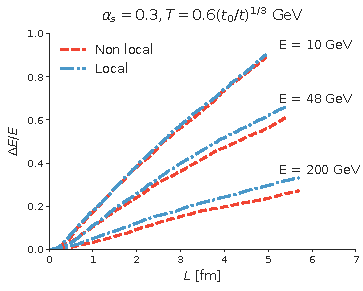
\includegraphics[width=\columnwidth]{Bjorken.pdf}
\caption{Energy loss fraction $\Delta E /E$ as function of path length $L$ at three different energies. Reddashed lines are direct simulations (the non-local case) and blue-dash-dotted lines are results using local approximation.}
\label{fig:Bjorken}
\end{figure}
Before applying this ``Modified rescattering" implementation of transport of energetic parton to heavy ion collisions, there are still a few issues we need to study and address.
The first issue concerns with the coherence effect in an expanding medium. 
The QGP produced in colliders only exists for a short amount of time and it undergoes violent expansion, i.e, the medium temperature may have changed notably during the formation time.
Therefore, we expect different radiation spectrum and correspondingly different amount of energy loss between the following two computing scenarios:
\begin{itemize}
\item[1.]  {\it A non-local (direct) calculation}: radiated gluons can precept the changing medium within the formation times.
\item[2.] {\it A local approximation}: calculate with rates obtained in the infinite medium defined by the local temperature at the radiation vertex.
\end{itemize} 
Although a non-local scenario should be more realistic, we would like to see how close the local approximation is.
We set-up simulations in medium that undergoes Bjorken expansion at mid-rapidity \cite{PhysRevD.27.140}. 
The temperature decreases with proper time,
\begin{eqnarray}
T(\Delta\tau) = T_0 \left(\frac{\tau_0}{\tau_0+\Delta\tau}\right)^{\frac{1}{3}}.
\end{eqnarray}
We chose $T_0=0.6$ GeV, $\tau_0=0.6$ fm/c and used a fixed coupling constant $\alpha_s = 0.3$.
The ``Modified Rescattering" approach is already a non-local calculation. because it preforms gluon rescatterings at different space-time during the evolution. 
To mimic the local approximation, we let each pre-gluon $i$ remember the temperature $T_i$ when it is first created and then perform rescatterings in an ``imaginary medium" defined by $T_i$.
The results are shown in Figure \ref{fig:Bjorken}. 
The difference between the two scenarios are negligible for low energy partons and is only moderate for a 200 GeV quark.
This is because for $\alpha_s = 0.3$ and the range of energy we considered, the maximum formation time $\sqrt{E/\hat{q}}$ is still small compared to the inverse of temperature changing rate $d\ln(T)/dt$.

\begin{figure}
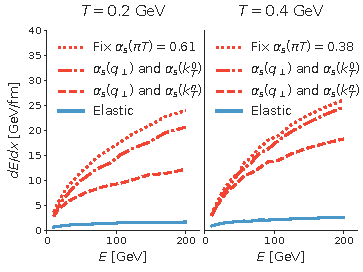
\includegraphics[width=\columnwidth]{Eloss_infinite_run.pdf}
\caption{Testing running coupling effect }
\label{fig:run}
\end{figure}
Second, we improve the previous calculation with a running coupling constant, following the prescription described in \cite{Arnold:2008zu}.
This involves two changes in the formula. 
For elastic scattering vertices, $\alpha_{s, \textrm{el}}$ is evaluated at the momentum transfer squared. 
This is already the feature of {\tt Lido} with running coupling.
For splitting vertices,  $\alpha_{s, \textrm{rad}}$ is evaluated at the final gluon transverse momenta squared,
\begin{eqnarray}\label{eq:kTn}
k_{\perp,n}^2 = \left(\vec{k}_T^0+\vec{q}_1+\cdots+\vec{q}_n\right)^2.
\end{eqnarray} 
In the {\tt Lido} model, the original scale used for $\alpha_{s, \textrm{rad}}$ is $k_{\perp,0}^2$ of the $2\rightarrow 3$ process.
Therefore, we change the acceptance probability $p$ for the running coupling version from the one in Step 3.2 to,
\begin{eqnarray}
p' = \min\left\{1, \frac{\tilde{\lambda}}{\tau_n}\times\frac{\alpha_s(k_{\perp,n})}{\alpha_s(k_{\perp,0})}\right\}
\end{eqnarray}
to include the running of the splitting vertices.
We can estimated the order of magnitude of $k_{\perp,n}^2$ to be $\sqrt{\hat{q}\omega}$ and it is about $\sqrt{\omega/T}$ times larger than the $k_{\perp,0}^2$ for gluons in the LPM region, therefore the running coupling effect suppress the spectrum by another factor of $\alpha_s(k_{\perp,n})/\alpha_s(k_{\perp,0})$.
In Figure. \ref{fig:run}, we showed three calculations in a static medium. The dotted lines uses a fixed coupling constant evaluated at a thermal scale $\alpha_s = \alpha_s((2\pi T)$.
This scale is also the lowest scale cut-off for the running coupling constant in our model (note that this minimum scale is not required in the original work \cite{Arnold:2008zu}).
The dash-dotted lines are running coupling calculations where the $\alpha_s(Q)$ of elastic process evaluated at $t$-channel momentum transfer and the $\alpha_s(Q)$ of the radiation vertex evaluated at $k_{T,0}^2$.
The dashed lines are also running coupling calculations but evaluate radiation $\alpha_s(Q)$ at $Q^2 = k_{\perp,n}^2$ through the modified acceptance probability $p'$.
The running coupling effect results in a reduction of the radiative energy loss.

\begin{figure}
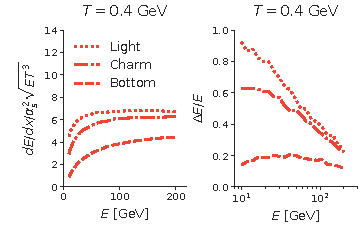
\includegraphics[width=\columnwidth]{Eloss_mass.pdf}
\caption{A demonstration of mass effect. Left plot: the scaled energy loss rate in an infinite medium for light quark, charm quark and bottom quark. Right plot: energy loss fraction of light quark, charm quark and bottom quark at path length $L=4$ fm, $\alpha_s(2\pi T) \approx 0.28$. }
\label{fig:mass}
\end{figure}

Finally, we put back the mass effects to study the heavy quark sector, including the massive particle kinematics, the formation time of gluon from a massive quark,
\begin{eqnarray}
\tau_{f} = \frac{2x(1-x)E}{k_\perp^2 + x^2M^2 + (1-x)m_g^2},
\end{eqnarray}
and the so-called ``dead-cone" effect where collinear radiations with angles $\theta \sim k_\perp/k < M/E$ are suppressed. 
The massive version of the $2\rightarrow3$ improved Gunion-Bertsch matrix-element has been derived in \cite{Uphoff:2014hza}; however, we have shown that on average rescatterings increases $k_{\perp}^2$, so a direct use of this massive $2\rightarrow3$ matrix-element in the ``Modified rescattering" approach leads to an unduly strong dead-cone effect.
The solution is to use the $2\rightarrow3$ matrix-element without mass effect to generate initial gluons, while implementing the dead-cone suppression in another factor of the gluon acceptance probability,
\begin{eqnarray}
p'' = \min\left\{1, \frac{\tilde{\lambda}}{\tau_n}\frac{\alpha_s(k_{\perp,n}^2)}{\alpha_s(k_{\perp,0}^2)} \left(\frac{k_{\perp,n}^2}{k_{\perp,n}^2+x^2 M^2}\right)^2\right\}.
\end{eqnarray}
On the left of Figure \ref{fig:mass}, the scaled energy loss rate in an infinite medium is extracted from simulations for light (massless), charm ($M=1.3$ GeV) and bottom ($M=4.2$ GeV) quarks. 
On the right, it is the energy loss fraction at a finite path-length $L=4$ fm.
In both cases, the mass introduces the energy loss ordering, $\Delta E_{\textrm{light}} > \Delta E_c > \Delta E_b$ and the differences decrease at higher energy.

\section{Summary and outlook}\label{section:summary}
To reduces the theory uncertainty introduced in the numerical implementation of the perturbative QCD transport of hard partons inside a quark-gluon plasma, we studied three different Monte-Carlo implementations and systematically compare them to the semi-analytic forms of parton energy loss.
We showed that the ``Modified Rescattering" approach well reproduces the coupling constant, temperature, parton energy and path-length dependences of the theoretical formula in both infinite- and thin-medium limits.
It also agrees with the predicted gluon spectrum within controlled uncertainty.
The expanding medium effect and running coupling effect are studied. For the application to the heavy-flavor sector, a tentative dead-cone effect implementation is proposed.
This approach is not restricted to scattering rate based model, it also applies to a diffusion modeling of the elastic processes. 
For future studies, controlling the uncertainties between Monte-Carlo implementation and theory can help us to perform a more unambiguous examination of theory assumptions and a more meaningful phenomenology extraction of jet, heavy quark transport properties in model-to-data comparisons.
Moreover, a Monte-Carlo generator that is tuned to match leading order theory calculation could be a good starting point to implement next-to-leading-order effects in the phenomenology models.

\begin{acknowledgments}
SAB and WK  are supported by the U.S. Department of Energy Grant no. DE-FG02-05ER41367. WK is also supported by NSF grant OAC-1550225.
\end{acknowledgments}

\begin{appendices}
\section{Gunion-Bertsch rate in the small momentum transfer limit}\label{app:consistency}
\section{A mored detailed comparison of radiation spectra}\label{app:tune-spectrum}
In Figure \ref{fig:spectrum} we examine the spectrum for at a single coupling and a single energy in an infinite medium. To evaluate the full performance of the Monte-Carlo, this appendix section provides detailed comparison at different energy, couplings and medium size.
\begin{figure}
\includegraphics[width=\columnwidth]{spectrum_E_alphas0d1.pdf}
\caption{The ratios of Monte-Carlo simulated spectra to the AMY NLL spectra (gray bands) and to the Gunion-Bertsch incoherent spectra (blue lines) are plotted, using $\alpha_s = 0.1$. The quark energy $E$ is 10, 50, 100, and 500 GeV as indicated by the rightmost vertical dashed lines in each subplots. The horizontal dashed lines denote $\pm 20\%$ deviation from unity.}
\label{fig:spectra-alphas=0.1}
\end{figure}

\begin{figure}
\includegraphics[width=\columnwidth]{spectrum_E_alphas0d3.pdf}
\caption{The same as Figure \ref{fig:spectra-alphas=0.1}, but for $\alpha_s = 0.3$.}
\label{fig:spectra-alphas=0.3}
\end{figure}

\label{app:tune}
\end{appendices}
\bibliography{mclpm} 
\end{document}